\documentclass{article}
\usepackage[utf8]{inputenc}
\usepackage{graphicx}
\usepackage{pgfplots}
\usepackage{amsmath}
\usepackage{amssymb}
\usepackage{amsfonts}
\usepackage{geometry}
\usepackage[thmmarks, amsmath, thref]{ntheorem}
\usepackage{mdframed}
\usepackage{amsthm}
\usepackage{physics}
\usepackage{proof}
\usepackage{derivative}
\usepackage{comment}
\usepackage{hyperref}
\usepackage{wrapfig}
\usepackage{amsthm}
\usepackage{xcolor}
\renewcommand{\theenumi}{\roman{enumi}}

\theoremstyle{nonumberplain}
\theoremheaderfont{\itshape}
\theorembodyfont{\upshape}
\theoremseparator{.}
\theoremsymbol{\ensuremath{\square}}
\theoremsymbol{\ensuremath{\blacksquare}}
\newtheorem{solution}{Solution}
\theoremseparator{. }
\theoremsymbol{\mbox{\texttt{;o)}}}

\pgfplotsset{compat=1.18}
\begin{document}

1. (2pts) El operador de interacción con un campo eléctrico \( \epsilon \) tiene la forma:
\[
\mu=-\mathbf{d} \cdot \epsilon
\]
donde \( \mathbf{d}=-e \mathbf{r} \) es el momento dipolar del electrón. Así, la tasa de transición entre estados \( |1\rangle \) y \( |2\rangle \) será proporcional al elemento de matriz:
\[
\langle 2| \mu|1\rangle
\]

Para \( \epsilon \) constante las transiciones estarán entonces mediadas por la expresión:
\[
\langle 2| \mathbf{r}|1\rangle
\]

Calcula la expresión 3 para el caso del pozo infinito unidimensional de longitud L con estados \( |m\rangle \) y \( |n\rangle \), y expresa en términos de los números cuánticos \( m \) y \( n \) la condición para las transiciones permitidas.

Queremos calcular

$$
\langle m | x | n \rangle = \int_0^L \psi_m(x) \, x \, \psi_n(x) \, dx
$$

Como las funciones de onda solución al pozo de potencial (con esta forma de pozo) que hemos visto son reales, podemos quitar el conjugado,

$$
\langle m | x | n \rangle = \frac{2}{L} \int_0^L \sin\left(\frac{m \pi x}{L}\right) x \sin\left(\frac{n \pi x}{L}\right) dx
$$

Utilizamos la identidad trigonométrica

$$
\sin A \sin B = \frac{1}{2} [\cos(A - B) - \cos(A + B)]
$$

Aplicamos

$$
\sin\left(\frac{m \pi x}{L}\right) \sin\left(\frac{n \pi x}{L}\right) = \frac{1}{2} \left[ \cos\left( \frac{(m - n)\pi x}{L} \right) - \cos\left( \frac{(m + n)\pi x}{L} \right) \right]
$$

Entonces,

$$
\langle m | x | n \rangle = \frac{1}{L} \int_0^L x \left[ \cos\left( \frac{(m - n)\pi x}{L} \right) - \cos\left( \frac{(m + n)\pi x}{L} \right) \right] dx
$$

Evaluamos ambas integrales por separado. Primero el caso general $m \neq n$ \\

Sea $k = \frac{(m \pm n)\pi}{L}$. Por Cálculo 2 sebemos que:

$$
\int_0^L x \cos(k x) dx = \left[ \frac{\cos(k x)}{k^2} + \frac{x \sin(k x)}{k} \right]_0^L
$$

Evaluamos para $I_{+} = \int_0^L x \cos\left( \frac{(m + n)\pi x}{L} \right) dx$ \\

Sea:

$$
k_+ = \frac{(m + n)\pi}{L}
$$

Entonces:

$$
I_{+} = \left[ \frac{\cos(k_+ x)}{k_+^2} + \frac{x \sin(k_+ x)}{k_+} \right]_0^L
$$

Evaluamos en los extremos: \\
En $x = 0$: $\cos(0) = 1$, $\sin(0) = 0$ \\
En $x = L$: \\
  $\cos(k_+ L) = \cos((m+n)\pi) = (-1)^{m+n}$ \\
  $\sin(k_+ L) = \sin((m+n)\pi) = 0$ \\

Entonces:

$$
I_{+} = \left[ \frac{(-1)^{m+n}}{k_+^2} + 0 \right] - \left[ \frac{1}{k_+^2} + 0 \right] = \frac{(-1)^{m+n} - 1}{k_+^2}
$$

Para $I_{-} = \int_0^L x \cos\left( \frac{(m - n)\pi x}{L} \right) dx$ \\

Digamos

$$
k_- = \frac{(m - n)\pi}{L}
$$

Evaluamos como antes:

$$
I_{-} = \left[ \frac{\cos(k_- x)}{k_-^2} + \frac{x \sin(k_- x)}{k_-} \right]_0^L
$$

En $x = 0$: $\cos(0) = 1$, $\sin(0) = 0$ \\
En $x = L$: \\
$\cos(k_- L) = \cos((m - n)\pi) = (-1)^{m-n}$ \\
$\sin(k_- L) = \sin((m - n)\pi) = 0$ \\

Entonces:

$$
I_{-} = \left[ \frac{(-1)^{m-n}}{k_-^2} + 0 \right] - \left[ \frac{1}{k_-^2} + 0 \right] = \frac{(-1)^{m-n} - 1}{k_-^2}
$$

Sustituimos en la expresión original:

$$
\langle m | x | n \rangle = \frac{1}{L} \left( I_{-} - I_{+} \right)
$$

$$
= \frac{1}{L} \left( \frac{(-1)^{m-n} - 1}{k_-^2} - \frac{(-1)^{m+n} - 1}{k_+^2} \right)
$$

Recordando que $k_{\pm} = \frac{(m \pm n)\pi}{L} \Rightarrow k_{\pm}^2 = \frac{(m \pm n)^2 \pi^2}{L^2}$ \\

Entonces:

$$
\langle m | x | n \rangle = \frac{1}{L} \left( \frac{(-1)^{m-n} - 1}{\left( \frac{(m - n)^2 \pi^2}{L^2} \right)} - \frac{(-1)^{m+n} - 1}{\left( \frac{(m + n)^2 \pi^2}{L^2} \right)} \right)
$$

Multiplicamos numerador y denominador para simplificar:

$$
\langle m | x | n \rangle = \frac{L^2}{\pi^2 L} \left( \frac{(-1)^{m-n} - 1}{(m - n)^2} - \frac{(-1)^{m+n} - 1}{(m + n)^2} \right)
$$

$$
\Rightarrow 
\langle m | x | n \rangle = \frac{L}{\pi^2} \left( \frac{(-1)^{m-n} - 1}{(m - n)^2} - \frac{(-1)^{m+n} - 1}{(m + n)^2} \right)
$$

Recordemos que $(-1)^k - 1 = 0$ si $k$ es par y $-2$ si $k$ es impar. Por tanto, ambos términos serán cero si $m \pm n$ es par. La contribución no nula ocurre si $m+n$ o $m-n$ es impar, es decir, cuando $m$ y $n$ tienen paridades opuestas; el caso de $m=n$ es trivial, pues el valor esperado está justamente al centro del pozo de potencial por simetría.

Por tanto, la condición para que $\langle m | x | n \rangle \neq 0$ (transición permitida):

$$
m + n \text{ impar} \quad o \quad m=n \quad \Rightarrow \quad m \text{ y } n \text{ iguales o de paridad opuesta}
$$


2. (3pts) La función de onda para el estado base del átomo de hidrógeno es
\[
\psi_{100}(r, \theta, \phi)=\frac{1}{\sqrt{\pi a^{3}}} e^{-r / a}
\]
donde
\[
a \equiv \frac{4 \pi \epsilon_{0} \hbar^{2}}{m_{e} e^{2}}=0,529 \times 10^{-10} \mathrm{~m}
\]
es el radio de Bohr. \\
a) Encuentre el valor esperado de \( r \) calculando \( \langle r\rangle=4 \pi \int_{0}^{\infty} \psi_{100}^{} r \psi_{100} r^{2} d r \). \\
b) Encuentre ahora el valor más probable de \( r \). Recuerde que la probabilidad de encontrar al electrón en el intervalo \( r \) a \( r+d r \) está dado por \( P=|\psi(r)|^{2} 4 \pi r^{2} d r \). \\
c) ¿Cuál sería ahora la probabilidad de que un electrón en el estado base se encuentre dentro del núcleo? Calcula primero la respuesta exacta asumiendo que la función de onda ec. 4 es correcta en el límite \( r=0 \) y denotando por \( b \) al radio del núcleo. \\
d) Expande tu resultado en una serie de potencias en términos del factor \( \epsilon=2 b / a \) (el cual es muy pequeño) y muestra que el término de orden más bajo es \( P \approx(4 / 3)(b / a)^{3} \). Calcula \( P \) con los valores \( b \approx 10^{-15} \mathrm{~m} \) y \( a \approx 0,5 \times 10^{-10} \mathrm{~m} \). De manera burda, esto representa la fracción de tiempo que el electrón se encuentra dentro del núcleo. \\

a) Trabajaremos en coordenadas esféricas, donde el volumen infinitesimal es $dV = r^2 \sin\theta \, dr \, d\theta \, d\phi$, y por simetría esférica podemos integrar únicamente sobre $r$. El valor esperado de $r$ se calcula como:

$$
\langle r \rangle = \int_{\mathbb{R}^3} \psi^ r \psi \, dV = \int_0^\infty \int_0^\pi \int_0^{2\pi} \psi^ r \psi \, r^2 \sin\theta \, d\phi \, d\theta \, dr
$$

Ya que la función es independiente de $\theta, \phi$, las integrales angulares dan $4\pi$, así que,

$$
\langle r \rangle = 4\pi \int_0^\infty \left| \psi_{100}(r) \right|^2 r^3 \, dr
$$

Sustituyendo la función:

$$
|\psi_{100}(r)|^2 = \frac{1}{\pi a^3} e^{-2r/a}
$$

Por tanto

$$
\langle r \rangle = \frac{4\pi}{\pi a^3} \int_0^\infty r^3 e^{-2r/a} dr = \frac{4}{a^3} \int_0^\infty r^3 e^{-2r/a} dr
$$

Hacemos el cambio de variable:

$$
u = \frac{2r}{a} \Rightarrow r = \frac{a u}{2}, \quad dr = \frac{a}{2} du
$$

$$
r^3 dr = \left(\frac{a u}{2}\right)^3 \frac{a}{2} du = \frac{a^4 u^3}{16} du
$$

Entonces,

$$
\langle r \rangle = \frac{4}{a^3} \cdot \int_0^\infty \frac{a^4 u^3}{16} e^{-u} du = \frac{4 a}{16} \int_0^\infty u^3 e^{-u} du
$$

La integral es la definición de la función gamma,

$$
\int_0^\infty u^3 e^{-u} du = \Gamma(4) = 3! = 6
$$

Finalmente:

$$
\langle r \rangle = \frac{a}{4} \cdot 6 = \frac{3a}{2}
$$

b) Valor más probable de $r$ \\

La densidad de probabilidad radial (al integrar sobre ángulos) es

$$
P(r) dr = |\psi_{100}(r)|^2 \cdot 4\pi r^2 \, dr = \frac{4}{a^3} r^2 e^{-2r/a} dr
$$

Para encontrar el valor más probable, maximizamos la función:

$$
f(r) = r^2 e^{-2r/a}
$$

Derivamos...

$$
\frac{df}{dr} = 2r e^{-2r/a} - \frac{2}{a} r^2 e^{-2r/a} = e^{-2r/a} \left(2r - \frac{2r^2}{a} \right)
$$

Igualamos a cero,

$$
e^{-2r/a} \left( 2r - \frac{2r^2}{a} \right) = 0 \Rightarrow 2r \left(1 - \frac{r}{a} \right) = 0
$$

Las soluciones son $r = 0$, $r = a$. Solo $r = a$ es un máximo (verificando que el valor mínimo de la función antes de derivar está asociado a cero).

$$
r_{\text{más probable}} = a
$$

c) La probabilidad de que el electrón esté dentro del núcleo (\( r < b \)) se calcula como:
\[
P = \int_{r=0}^{b} |\psi_{100}(r)|^2  4\pi r^2  dr
\]
Sustituyendo \( |\psi_{100}(r)|^2 = \frac{1}{\pi a^3} e^{-2r/a} \):
\[
P = \frac{4}{a^3} \int_0^b r^2 e^{-2r/a}  dr
\]
La integral se resuelve usando la fórmula para \( \int_0^b r^n e^{-\lambda r}  dr \) con \( n=2 \), \( \lambda = \frac{2}{a} \):
\[
\int_0^b r^2 e^{-\lambda r}  dr = \frac{2}{\lambda^3} \left[ 1 - e^{-\lambda b} \left( 1 + \lambda b + \frac{(\lambda b)^2}{2} \right) \right]
\]
Sustituyendo \( \lambda = \frac{2}{a} \):
\[
\int_0^b r^2 e^{-2r/a}  dr = \frac{a^3}{4} \left[ 1 - e^{-2b/a} \left( 1 + \frac{2b}{a} + \frac{2b^2}{a^2} \right) \right]
\]
Por lo tanto:
\[
P = \frac{4}{a^3} \cdot \frac{a^3}{4} \left[ 1 - e^{-2b/a} \left( 1 + \frac{2b}{a} + \frac{2b^2}{a^2} \right) \right] = 1 - e^{-2b/a} \left( 1 + \frac{2b}{a} + \frac{2b^2}{a^2} \right)
\]

d) Expansión en serie de potencias para \( \epsilon = \frac{2b}{a} \ll 1 \)

   Definimos \( \epsilon = \frac{2b}{a} \). La probabilidad es:
   \[
   P = 1 - e^{-\epsilon} \left( 1 + \epsilon + \frac{\epsilon^2}{2} \right)
   \]
   Expandimos \( e^{-\epsilon} \) hasta \( \mathcal{O}(\epsilon^4) \):
   \[
   e^{-\epsilon} = 1 - \epsilon + \frac{\epsilon^2}{2} - \frac{\epsilon^3}{6} + \frac{\epsilon^4}{24} + \cdots
   \]
   Multiplicamos por \( \left( 1 + \epsilon + \frac{\epsilon^2}{2} \right) \):
   \[
   e^{-\epsilon} \left( 1 + \epsilon + \frac{\epsilon^2}{2} \right) = \left(1 - \epsilon + \frac{\epsilon^2}{2} - \frac{\epsilon^3}{6} + \cdots \right) \left(1 + \epsilon + \frac{\epsilon^2}{2} \right)
   \]
   Los términos hasta \( \epsilon^3 \): \\
   - Constante: \( 1 \cdot 1 = 1 \) \\
   - Lineal: \( 1 \cdot \epsilon + (-\epsilon) \cdot 1 = 0 \) \\
   - Cuadrático: \( 1 \cdot \frac{\epsilon^2}{2} + (-\epsilon) \cdot \epsilon + \frac{\epsilon^2}{2} \cdot 1 = 0 \) \\
   - Cúbico: \( (-\epsilon) \cdot \frac{\epsilon^2}{2} + \frac{\epsilon^2}{2} \cdot \epsilon + \left(-\frac{\epsilon^3}{6}\right) \cdot 1 = -\frac{\epsilon^3}{6} \) 
   \[
   \implies e^{-\epsilon} \left( 1 + \epsilon + \frac{\epsilon^2}{2} \right) = 1 - \frac{\epsilon^3}{6} + \mathcal{O}(\epsilon^4)
   \]
   Sustituyendo:
   \[
   P = 1 - \left( 1 - \frac{\epsilon^3}{6} + \cdots \right) = \dfrac{\epsilon^3}{6} + \mathcal{O}(\epsilon^4)
   \]
  
   Para \( r \ll a \), aproximamos \( e^{-2r/a} \approx 1 - \frac{2r}{a} + \frac{2r^2}{a^2} \):
   \[
   P \approx \frac{4}{a^3} \int_0^b r^2 \left( 1 - \frac{2r}{a} + \frac{2r^2}{a^2} \right) dr
   \]
   Resolviendo la integral:
   \[
   \int_0^b r^2  dr = \frac{b^3}{3}, \quad \int_0^b r^3  dr = \frac{b^4}{4}, \quad \int_0^b r^4  dr = \frac{b^5}{5}
   \]
   \[
   P \approx \frac{4}{a^3} \left( \frac{b^3}{3} - \frac{2}{a} \cdot \frac{b^4}{4} + \frac{2}{a^2} \cdot \frac{b^5}{5} \right) = \frac{4}{3} \left( \frac{b}{a} \right)^3 - 2 \left( \frac{b}{a} \right)^4 + \frac{8}{5} \left( \frac{b}{a} \right)^5
   \]
   El término dominante es:
   \[
   P \approx \dfrac{4}{3} \left( \dfrac{b}{a} \right)^3
   \]

Como \( b \approx 10^{-15}  \text{m} \) y \( a \approx 0.5 \times 10^{-10}  \text{m} \):
   \[
   \frac{b}{a} = \frac{10^{-15}}{5 \times 10^{-11}} = 2 \times 10^{-5}, \quad \left( \frac{b}{a} \right)^3 = 8 \times 10^{-15}
   \]
   \[
   P \approx \frac{4}{3} \times 8 \times 10^{-15} = 1.067 \times 10^{-14}
   \]


3. (3pts) La parte radial de la ecuación de Schödinger en su forma unidimensional puede ser escrita como:
\[
\frac{-\hbar^{2}}{2 m} \frac{d^{2} P_{n l}}{d r^{2}}+U_{l}(r) P_{n l}=E_{n} P_{n l}
\]
donde
\[
U_{l}(r)=-\frac{Z e^{2}}{4 \pi \epsilon_{0} r}+\frac{\hbar^{2}}{2 m} \frac{l(l+1)}{r^{2}}
\]
es la energía potencial efectiva.\\
a) Grafica \( U_{l}(r) \) como función de \( x=Z r / a_{0} \) para \( l=1 \).\\
b) Encuentra una expresión en términos de \( n \) y \( l \neq 0 \) para aquellos valores de \( x \) para los cuales \( E_{n}=U_{l}(r) \). Estos valores \( x_{1} \) y \( x_{2} \) son llamados puntos de retorno clásicos. Una partícula clásica estaría confinada a la región definida entre estos puntos. Evalúa \( x_{1} \) y \( x_{2} \) para \( n=3 \) y \( l=1 \).\\
c) Muestra que dentro del rango \( x_{1}<x<x_{2} \) la función de onda \( P_{n l} \) es cóncava hacia el eje \( x \), pero fuera de éste, \( P_{n l} \) es convexo hacia el eje \( x \).\\
d) ¿Cuántos nodos tiene la función \( P_{31} \) ?. Muestra que todos los nodos de \( P_{n l} \) deben yacer dentro de la región clásica \( x_{1}<x<x_{2} \).\\
e) Repite el problema para \( n=3, l=0 \) y discuta las diferencias entre los casos \( l=0 \) y \( l \neq 0 \).\\

a) Gráfica del potencial efectivo $U_l(r)$ para $l = 1$

\begin{figure}[h]
    \centering
    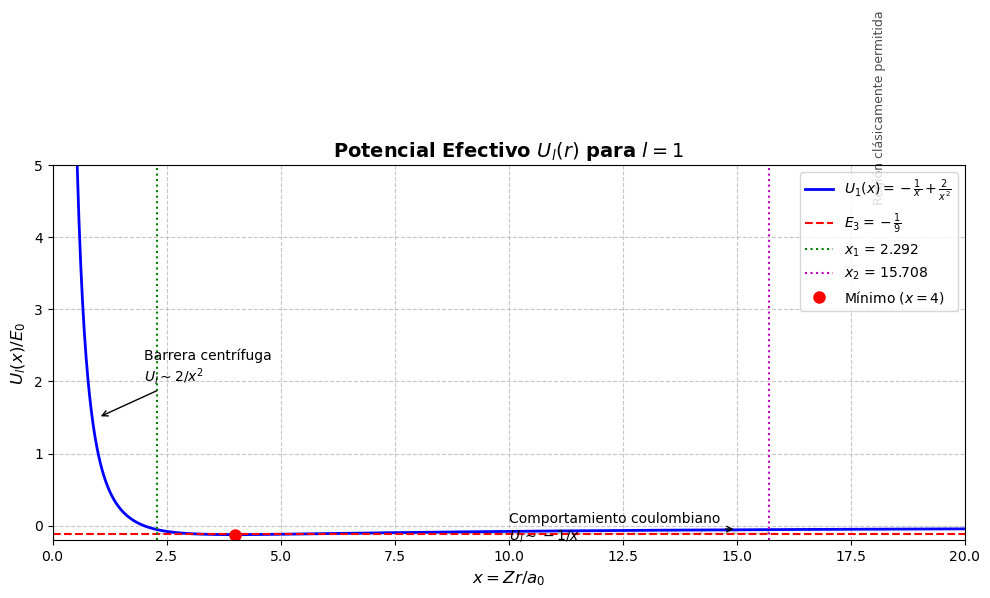
\includegraphics[width=0.75\linewidth]{Graphic.png}
    \caption{Grafico del inciso a)}
    \label{fig:enter-label}
\end{figure}

b) Puntos de retorno clásicos $x_1, x_2$ tal que $E_n = U_l(r)$

La condición para los puntos de retorno es:

$$
E_n = U_l(r)
$$

Para el átomo de hidrógeno, la energía en el estado $n$ es:

$$
E_n = -\frac{Z^2 e^2}{8 \pi \varepsilon_0 a_0 n^2}
$$

Y en unidades adimensionales $x = Zr/a_0$, transformamos:

$$
U_l(r) = -\frac{e^2}{4 \pi \varepsilon_0 r} + \frac{\hbar^2 l(l+1)}{2 m r^2}
= \frac{Z^2 e^2}{4 \pi \varepsilon_0 a_0} \left( -\frac{1}{x} + \frac{l(l+1)}{x^2} \right)
$$

La energía también se expresa en unidades del Rydberg:

$$
E_n = - \frac{Z^2 e^2}{8 \pi \varepsilon_0 a_0 n^2}
$$

Entonces:

$$
E_n = \frac{Z^2 e^2}{4 \pi \varepsilon_0 a_0} \cdot \left( -\frac{1}{2n^2} \right)
$$

Igualamos:

$$
- \frac{1}{2n^2} = -\frac{1}{x} + \frac{l(l+1)}{x^2}
$$

Multiplicamos todo por $x^2$:

$$
- \frac{x^2}{2n^2} = -x + l(l+1)
\quad \Rightarrow \quad
\frac{x^2}{2n^2} - x + l(l+1) = 0
$$

Esta es una ecuación cuadrática en $x$, que resolvemos:

$$
x^2 - 2n^2 x + 2n^2 l(l+1) = 0
$$

Solución:

$$
x_{1,2} = n^2 \left(1 \pm \sqrt{1 - \frac{2 l(l+1)}{n^2}} \right)
$$

Para $n=3, l=1$:

$$
x_{1,2} = 9 \left(1 \pm \sqrt{1 - \frac{2\cdot2}{9}} \right)
= 9 \left(1 \pm \sqrt{1 - \frac{4}{9}} \right)
= 9 \left(1 \pm \sqrt{\frac{5}{9}} \right)
= 9 \left(1 \pm \frac{\sqrt{5}}{3} \right)
$$

$$
x_1 = 9 \left(1 - \frac{\sqrt{5}}{3} \right), \quad
x_2 = 9 \left(1 + \frac{\sqrt{5}}{3} \right)
$$

Valor numérico:

$$
\sqrt{5} \approx 2.236 \Rightarrow
x_1 \approx 9 (1 - 0.745) \approx 9 \cdot 0.255 \approx 2.3
\quad
x_2 \approx 9 (1 + 0.745) \approx 9 \cdot 1.745 \approx 15.7
$$

$$
x_1 \approx 2.3, \quad x_2 \approx 15.7
$$

c) Concavidad de la función $P_{nl}(r)$ }}

Recordamos la ecuación radial unidimensional:

$$
\frac{-\hbar^{2}}{2 m} \frac{d^{2} P_{nl}}{d r^{2}} + U_l(r) P_{nl} = E_n P_{nl}
$$

Reescribiéndola como:

$$
\frac{d^2 P_{nl}}{d r^2} = \frac{2m}{\hbar^2} \left[ U_l(r) - E_n \right] P_{nl}
$$

Ahora analizamos el signo de la derivada segunda: //

Si $U_l(r) < E_n$, entonces $\frac{d^2 P}{dr^2} < 0$ cuando $P > 0$ \rightarrow \textit{cóncava hacia el eje } $r$. \\
Si $U_l(r) > E_n$, entonces $\frac{d^2 P}{dr^2} > 0$ cuando $P > 0$ \rightarrow \textit{convexa hacia el eje } $r$. \\

Trabajamos en términos de la variable adimensional.

$$
x = \frac{Zr}{a_0} \quad \Rightarrow \quad r = \frac{a_0}{Z} x
$$

Usamos:

$$
U_l(x) = E_0 \left( -\frac{1}{x} + \frac{l(l+1)}{x^2} \right), \quad E_n = -\frac{E_0}{n^2}, \quad E_0 = \frac{m e^4}{8 \varepsilon_0^2 h^2} = 13.6\, \text{eV}
$$

Entonces la ecuación en términos de $x$ se vuelve:

$$
\frac{d^2 P}{dx^2} = \frac{2m a_0^2}{\hbar^2 Z^2} \left[ U_l(x) - E_n \right] P
$$

Como $\frac{2ma_0^2}{\hbar^2 Z^2} > 0$, el signo de $\frac{d^2 P}{dx^2}$ viene determinado únicamente por el signo de $U_l(x) - E_n$.

d) Nodos de $P_{31}$ y su localización

La función $P_{nl}(r)$ tiene exactamente $n - l - 1$ nodos radiales (excluyendo el nodo en $r = 0$).

Para el caso $n = 3, l = 1$:

$$
\ \text{ nodos} = 3 - 1 - 1 = 1
$$

En mecánica cuántica de una dimensión efectiva, los nodos deben encontrarse donde la energía cinética es positiva, es decir:

$$
U_l(x) < E_n \quad \Rightarrow \quad x_1 < x < x_2
$$

Esto garantiza que el valor de $\frac{d^2 P}{dx^2}$ sea negativo (curvatura hacia abajo), lo cual permite que la función cruce el eje (es decir, tenga nodos reales). Fuera de esta región, la solución es exponencial y no puede oscilar, por lo que no puede haber nodos.

e) Comparación entre $(n = 3, l = 1)$ y $(n = 3, l = 0)$ \\

 Número de nodos: \\

 Para $n = 3, l = 1$: $3 - 1 - 1 = 1$ nodo. \\
 Para $n = 3, l = 0$: $3 - 0 - 1 = 2$ nodos. \\

 Forma del potencial efectivo: \\

Recordamos,

$$
U_l(r) = -\frac{1}{x} + \frac{l(l+1)}{x^2}
$$

 Para $l = 1$: aparece una barrera centrífuga positiva $\sim 2/x^2$ en el origen. \\
 Para $l = 0$: no hay término centrífugo $\Rightarrow$ el potencial es singular atractor puro $U_0(x) = -1/x$. \\

 En el caso $l = 0$, la función de onda no tiene ninguna barrera que le impida concentrarse cerca del núcleo, y puede penetrar profundamente. Los nodos se distribuyen más cercanos al origen. En el caso $l = 1$, la barrera centrífuga excluye la región cercana al origen (efecto de repulsión angular), por lo que el nodo y el pico de probabilidad están desplazados a mayores valores de $x$.

4. (2pts) Recordando las reglas de transición para el átomo de hidrógeno:

\[
\Delta l = \pm 1
\]
\[
\Delta m_l = 0, \pm 1
\]

a) Supongamos un electrón en el estado \(4p\). ¿A cuáles estados puede transicionar al radiar un fotón, según las reglas de selección?

b) Compruebe la regla de selección para \(n = 2 \to n = 1\), tomando la función de onda:

\[
\psi_{200}(r, \theta, \phi) = \frac{1}{4\sqrt{2\pi} a^{3/2}} \left(2 - \frac{r}{a}\right) e^{-r/2a}
\]

y calculando:

\[
4\pi \int_0^\infty \psi_{100} r \psi_{200} r^2 \, dr
\]


a= Sabemos que el estado $4p$ corresponde a: \\
$n = 4$ \\
$l = 1$ \\
$m_l \in \{-1, 0, 1\}$ \\

El sistema sufre una transición de dipolo eléctrico, y bajo esta interacción la perturbación relevante es proporcional al operador de posición $\vec{r}$. Esto impone restricciones sobre los posibles estados finales, conocidas como reglas de selección, que derivan del análisis de simetría (grupo de rotaciones y paridad). Dichas reglas son: \\

 $\Delta l = \pm 1$ \\
 $\Delta m_l = 0, \pm 1$ \\

Es decir, solo puede cambiar su momento angular orbital en una unidad y la componente proyectada también puede variar en una unidad o permanecer constante. Además, dado que el fotón transporta energía, el electrón necesariamente pasa a un nivel de menor energía, es decir, a un nivel con $n' < 4$. \\

Queremos entonces determinar todos los estados $(n', l')$ accesibles desde $(4, l=1)$ por medio de estas reglas. \\

Para cada $n' < 4$, escribimos los valores posibles de $l'$ que cumplen $|l - l'| = 1$, es decir, $l' = 0$ o $2$. Así: \\

 Si $n' = 3$, entonces $l' = 0$ y $2$ son estados permitidos $\Rightarrow$ $3s$, $3d$ \\
 Si $n' = 2$, entonces $l' = 0$ y $2$ también existen $\Rightarrow$ $2s$, $2d$ (creo que no incluye a 2d pero me voy a arriesgar xd) \\
 Si $n' = 1$, solo existe $l'=0$ $\Rightarrow$ $1s$ \\

Por lo tanto, los únicos estados accesibles por transición dipolar desde $4p$ son:

$$
3s,\quad 3d,\quad 2s,\quad 2d,\quad 1s
$$

Naturalmente, cada uno de estos estados tiene sus propios valores permitidos de $m_l'$, pero mientras alguno de ellos cumpla la condición $\Delta m_l = 0, \pm 1$, la transición es posible. \\

b) Verificación explícita de la regla de selección para $2s \to 1s$; nos dan la función de onda del estado $2s$, que es:

$$
\psi_{200}(r, \theta, \phi) = \frac{1}{4\sqrt{2\pi} a^{3/2}} \left(2 - \frac{r}{a}\right) e^{-r/2a}
$$

Este estado tiene $l = 0$, $m_l = 0$. La función de onda no depende de los ángulos, pues el armónico esférico correspondiente es $Y_0^0 = \frac{1}{\sqrt{4\pi}}$, constante. El estado final es el fundamental:

$$
\psi_{100}(r, \theta, \phi) = \frac{1}{\sqrt{\pi a^3}} e^{-r/a}
$$

Nuevamente, no depende de $\theta, \phi$, ya que es un estado $s$, con $l = 0$. Entonces la integral total del elemento de matriz del operador de posición se factoriza:

$$
\langle \psi_{100} | r | \psi_{200} \rangle = \int \psi_{100}^(\vec{r})\, r\, \psi_{200}(\vec{r})\, d^3r = \int_0^\infty \psi_{100}(r) \psi_{200}(r)\, r^3\, dr \cdot \int_{\Omega} |Y_0^0|^2 d\Omega
$$

Donde $\Omega$ denota la parte angular del volumen (es decir, $\theta, \phi$). Dado que ambos estados tienen $l=0$, el producto $Y_0^0 Y_0^0$ da $\frac{1}{4\pi}$, y su integral angular es:

$$
\int_{\Omega} \frac{1}{4\pi} d\Omega = \frac{1}{4\pi} \cdot 4\pi = 1
$$

Entonces, el problema se reduce al cálculo de una integral radial:

$$
\langle \psi_{100} | r | \psi_{200} \rangle = \int_0^\infty \psi_{100}(r) \psi_{200}(r)\, r^3\, dr
$$

Sustituyendo las expresiones dadas: \\

 $\psi_{100}(r) = \frac{1}{\sqrt{\pi a^3}} e^{-r/a}$ \\
 $\psi_{200}(r) = \frac{1}{4\sqrt{2\pi} a^{3/2}} \left(2 - \frac{r}{a} \right) e^{-r/2a}$ \\

Multiplicamos ambas y extraemos las constantes:

$$
\psi_{100}(r)\psi_{200}(r) = \frac{1}{4\sqrt{2}\pi a^3} \left(2 - \frac{r}{a} \right) e^{-3r/2a}
$$

Entonces:

$$
\langle \psi_{100} | r | \psi_{200} \rangle = \frac{1}{4\sqrt{2} \pi a^3} \int_0^\infty \left(2 - \frac{r}{a} \right) r^3 e^{-3r/2a} dr
$$

Esta integral contiene la información completa. Para evaluarla, cambio de variable: definamos $u = \frac{r}{a} \Rightarrow r = au,\ dr = a du$ \\

La integral se convierte en:

$$
= \frac{1}{4\sqrt{2} \pi a^3} \cdot a^4 \int_0^\infty (2 - u) u^3 e^{-3u/2} du = \frac{a}{4\sqrt{2} \pi} \int_0^\infty (2 - u) u^3 e^{-3u/2} du
$$

Ahora desarrollo la expresión bajo la integral:

$$
(2 - u) u^3 = 2u^3 - u^4
$$

Luego:

$$
\langle \psi_{100} | r | \psi_{200} \rangle = \frac{a}{4\sqrt{2} \pi} \left[ 2 \int_0^\infty u^3 e^{-3u/2} du - \int_0^\infty u^4 e^{-3u/2} du \right]
$$

Estas integrales son del tipo gamma:

$$
\int_0^\infty u^n e^{-\lambda u} du = \frac{n!}{\lambda^{n+1}}
$$

Con $\lambda = \frac{3}{2}$, obtenemos: \\

$\int_0^\infty u^3 e^{-3u/2} du = \frac{3!}{(3/2)^4} = \frac{6}{(81/16)} = \frac{96}{81} = \frac{32}{27}$ \\
$\int_0^\infty u^4 e^{-3u/2} du = \frac{4!}{(3/2)^5} = \frac{24}{(243/32)} = \frac{768}{243} = \frac{256}{81}$ \\

Entonces la integral vale:

$$
\langle \psi_{100} | r | \psi_{200} \rangle = \frac{a}{4\sqrt{2}\pi} \left( 2 \cdot \frac{32}{27} - \frac{256}{81} \right)
= \frac{a}{4\sqrt{2}\pi} \left( \frac{64}{27} - \frac{256}{81} \right)
= \frac{a}{4\sqrt{2}\pi} \cdot \left( \frac{192 - 256}{81} \right)
= \frac{a}{4\sqrt{2}\pi} \cdot \left( -\frac{64}{81} \right)
$$

Por tanto:

$$
\langle \psi_{100} | r | \psi_{200} \rangle = -\frac{16a}{81\sqrt{2}\pi} \neq 0
$$

Pero este resultado NO contradice la regla de selección, porque hemos calculado solo la parte radial del elemento de matriz. La transición inducida por $\vec{r}$ requiere evaluar el elemento completo:

$$
\langle 100 | \vec{r} | 200 \rangle = \int \psi_{100}(\vec{r})\, \vec{r} \, \psi_{200}(\vec{r})\, d^3r
$$

Esta integral es un vector, y su componente angular depende de $\int Y_0^{0}(\theta, \phi) \cos\theta\, Y_0^0(\theta, \phi)\, d\Omega$, es decir, una integral de un armónico esférico grado 0 contra $\cos\theta$, que es un armónico de $l = 1$. Por ortogonalidad:

$$
\int Y_0^0 \cdot Y_1^0\, d\Omega = 0
$$

Por tanto, aunque la integral radial es no nula, el producto total angular es cero, y la transición queda prohibida.

\end{document}

